% Complex Tori and Elliptic Curves --- A0 portrait academic poster.
% A NARRATED poster (not a book-map): it tells ONE story --- the chord-tangent law on a
% cubic IS addition on the torus C/Lambda, carried over by the Weierstrass functions ---
% motivating each step in words before symbols, with one worked example.
%
% Layout discipline (this revision fixes the earlier clipping/size mess):
%  * figures are sized by a UNIFORM HEIGHT (\figH) so their stroke and label weights match;
%  * the dependency diagram lives in its OWN full-width block, sized by height, so the block
%    grows to it and nothing overflows (the old side-by-side minipage made it clip);
%  * the header carries only text, in two balanced columns.
% Reuses the book's Sage figures and palette (figuremacros.tex mirrors ../book/preamble.tex;
% coordinates from ../sagemath).  Build:  pdflatex poster.tex  (twice).
\documentclass[25pt, a0paper, portrait, margin=14mm, innermargin=15mm,
               blockverticalspace=12mm, colspace=16mm, subcolspace=8mm]{tikzposter}

\usepackage{amsmath,amssymb,mathtools}

% figuremacros.tex --- figure infrastructure harvested from book/preamble.tex
% (TikZ libraries, the form* colour palette, the three \drawprecise macros,
%  and the diagram tikzset). Do not edit; mirror of the book's definitions.

\usetikzlibrary{arrows.meta,calc,positioning,decorations.markings,decorations.pathmorphing,
  patterns,shadings,shapes.geometric,fadings,backgrounds,intersections,bending}

\definecolor{formteal}{HTML}{1f4e79}
\definecolor{formgold}{HTML}{b88a14}
\definecolor{formrust}{HTML}{a8431d}
\definecolor{formplum}{HTML}{6b2e6e}
\definecolor{formsage}{HTML}{467b3a}
\definecolor{formslate}{HTML}{3a5168}
\definecolor{formivory}{HTML}{f6efe0}

\newcommand{\drawprecisetorus}{%
  % (1) Fill the visible torus body with light teal.
  \fill[formteal!13, line join=round]
    plot[smooth cycle] coordinates {\torusOuter};
  % (2) Cut out the donut hole using the inner silhouette curve.
  \fill[white, line join=round]
    plot[smooth cycle] coordinates {\torusInner};
  % (3) Visible meridian arcs (eight small circles spaced 45 deg apart).
  % Back meridians (v in [0, pi]) form one visible arc each;
  % front meridians (v in (pi, 2 pi)) wrap across u = 0 and are split
  % into two visible chunks (VA and VB) by the sampling boundary.
  \draw[draw=formteal!60!black, line width=0.42pt, line join=round, opacity=0.9]
    plot[smooth] coordinates {\torusMerZeroVA};
  \draw[draw=formteal!60!black, line width=0.42pt, line join=round, opacity=0.9]
    plot[smooth] coordinates {\torusMerOneVA};
  \draw[draw=formteal!60!black, line width=0.42pt, line join=round, opacity=0.9]
    plot[smooth] coordinates {\torusMerTwoVA};
  \draw[draw=formteal!60!black, line width=0.42pt, line join=round, opacity=0.9]
    plot[smooth] coordinates {\torusMerThreeVA};
  \draw[draw=formteal!60!black, line width=0.42pt, line join=round, opacity=0.9]
    plot[smooth] coordinates {\torusMerFourVA};
  \draw[draw=formteal!60!black, line width=0.42pt, line join=round, opacity=0.9]
    plot[smooth] coordinates {\torusMerFiveVA};
  \draw[draw=formteal!60!black, line width=0.42pt, line join=round, opacity=0.9]
    plot[smooth] coordinates {\torusMerFiveVB};
  \draw[draw=formteal!60!black, line width=0.42pt, line join=round, opacity=0.9]
    plot[smooth] coordinates {\torusMerSixVA};
  \draw[draw=formteal!60!black, line width=0.42pt, line join=round, opacity=0.9]
    plot[smooth] coordinates {\torusMerSixVB};
  \draw[draw=formteal!60!black, line width=0.42pt, line join=round, opacity=0.9]
    plot[smooth] coordinates {\torusMerSevenVA};
  \draw[draw=formteal!60!black, line width=0.42pt, line join=round, opacity=0.9]
    plot[smooth] coordinates {\torusMerSevenVB};
  % (4) Visible longitude arcs (the four canonical latitude circles).
  % Outer (u=0) is visible only on the front half (v in (pi, 2 pi)),
  % inner (u=pi) only on the back half (v in (0, pi)); the top crest
  % (u=pi/2) is visible everywhere; the bottom (u=3pi/2) is fully hidden.
  \draw[draw=formteal!60!black, line width=0.5pt, line join=round, opacity=0.95]
    plot[smooth] coordinates {\torusLonTopVA};
  \draw[draw=formteal!60!black, line width=0.42pt, line join=round, opacity=0.8]
    plot[smooth] coordinates {\torusLonOuterVA};
  \draw[draw=formteal!60!black, line width=0.42pt, line join=round, opacity=0.8]
    plot[smooth] coordinates {\torusLonInnerVA};
  % (5) Crisp silhouette outlines drawn last so they sit on top.
  \draw[draw=formteal!65!black, line width=0.95pt, line join=round]
    plot[smooth cycle] coordinates {\torusOuter};
  \draw[draw=formteal!65!black, line width=0.8pt, line join=round]
    plot[smooth cycle] coordinates {\torusInner};
}

\newcommand{\drawprecisesphere}{%
  % Color tone matches the torus (formteal) for visual unity across figures.
  % (1) Flat-filled body of the sphere (same filling style as the torus)
  \fill[formteal!13, line join=round]
    plot[smooth cycle] coordinates {\sphereOutline};
  % (2) Visible latitude arcs
  \draw[draw=formteal!60!black, line width=0.45pt, line join=round, opacity=0.9]
    plot[smooth] coordinates {\sphereLatEquatorVA};
  \draw[draw=formteal!60!black, line width=0.4pt, line join=round, opacity=0.85]
    plot[smooth] coordinates {\sphereLatNorthVA};
  \draw[draw=formteal!60!black, line width=0.4pt, line join=round, opacity=0.85]
    plot[smooth] coordinates {\sphereLatNorthVB};
  \draw[draw=formteal!60!black, line width=0.4pt, line join=round, opacity=0.85]
    plot[smooth] coordinates {\sphereLatTropicVA};
  \draw[draw=formteal!60!black, line width=0.4pt, line join=round, opacity=0.85]
    plot[smooth] coordinates {\sphereLatTropicVB};
  \draw[draw=formteal!60!black, line width=0.4pt, line join=round, opacity=0.85]
    plot[smooth] coordinates {\sphereLatSouthVA};
  % (3) Visible meridian arcs (eight meridians at v = k pi/4)
  \draw[draw=formteal!60!black, line width=0.42pt, line join=round, opacity=0.9]
    plot[smooth] coordinates {\sphereMerZeroVA};
  \draw[draw=formteal!60!black, line width=0.42pt, line join=round, opacity=0.9]
    plot[smooth] coordinates {\sphereMerOneVA};
  \draw[draw=formteal!60!black, line width=0.42pt, line join=round, opacity=0.9]
    plot[smooth] coordinates {\sphereMerTwoVA};
  \draw[draw=formteal!60!black, line width=0.42pt, line join=round, opacity=0.9]
    plot[smooth] coordinates {\sphereMerThreeVA};
  \draw[draw=formteal!60!black, line width=0.42pt, line join=round, opacity=0.9]
    plot[smooth] coordinates {\sphereMerFourVA};
  \draw[draw=formteal!60!black, line width=0.42pt, line join=round, opacity=0.9]
    plot[smooth] coordinates {\sphereMerFiveVA};
  \draw[draw=formteal!60!black, line width=0.42pt, line join=round, opacity=0.9]
    plot[smooth] coordinates {\sphereMerSixVA};
  \draw[draw=formteal!60!black, line width=0.42pt, line join=round, opacity=0.9]
    plot[smooth] coordinates {\sphereMerSevenVA};
  % (4) Hidden back arcs as dashed light strokes
  \draw[draw=formteal!50!black, dashed, line width=0.3pt, line join=round, opacity=0.55]
    plot[smooth] coordinates {\sphereLatEquatorHA};
  % (5) Crisp silhouette outline on top
  \draw[draw=formteal!65!black, line width=0.95pt, line join=round]
    plot[smooth cycle] coordinates {\sphereOutline};
}

\newcommand{\drawprecisecurve}{%
  % Oval (compact component, x in [-1,0]): draw as closed smooth cycle.
  \draw[draw=formteal!60!black, line width=0.88pt, line join=round]
    plot[smooth cycle, tension=0.85] coordinates {\curveOvalFull};
  % Branch (unbounded component, x >= 1): upper and lower arcs.
  \draw[draw=formteal!60!black, line width=0.88pt, line join=round]
    plot[smooth, tension=0.9] coordinates {\curveBranchUpper};
  \draw[draw=formteal!60!black, line width=0.88pt, line join=round]
    plot[smooth, tension=0.9] coordinates {\curveBranchLower};
  % Branch points (Weierstrass roots e1=-1, e2=0, e3=1)
  \fill[formteal!70!black] (-1,0) circle (1.8pt);
  \fill[formteal!70!black] ( 0,0) circle (1.8pt);
  \fill[formteal!70!black] ( 1,0) circle (1.8pt);
}

\tikzset{
  arrow/.style={-{Latex[length=2mm]}, thick},
  point/.style={circle, fill=black, inner sep=1.5pt},
  labelnode/.style={font=\small, align=center},
  note/.style={draw=black!55, rounded corners=2pt, align=center, inner sep=5pt, fill=black!3},
  visualnode/.style={draw=black!60, rounded corners=2pt, align=center, inner sep=6pt, fill=black!2}
}


\newcommand{\C}{\mathbb{C}}
\newcommand{\R}{\mathbb{R}}
\newcommand{\Z}{\mathbb{Z}}
\newcommand{\Q}{\mathbb{Q}}
\newcommand{\F}{\mathbb{F}}
\newcommand{\CP}{\mathbb{CP}}
\newcommand{\HH}{\mathbb{H}}
\newcommand{\Pic}{\operatorname{Pic}}
\newcommand{\ord}{\operatorname{ord}}

\newcommand{\sagedir}{../sagemath}
\input{\sagedir/coords.tex}
\input{\sagedir/coords_torus.tex}
\input{\sagedir/coords_curve_sample.tex}

\definecolorstyle{book}{}{%
  \colorlet{backgroundcolor}{formivory!55}%
  \colorlet{framecolor}{formteal!70!black}%
}{%
  \colorlet{titlefgcolor}{formivory}%
  \colorlet{titlebgcolor}{formteal!88!black}%
}{%
  \colorlet{blocktitlebgcolor}{formteal}%
  \colorlet{blocktitlefgcolor}{white}%
  \colorlet{blockbodybgcolor}{white}%
  \colorlet{blockbodyfgcolor}{black}%
}{%
  \colorlet{innerblocktitlebgcolor}{formgold}%
  \colorlet{innerblocktitlefgcolor}{black}%
  \colorlet{innerblockbodybgcolor}{formgold!18}%
  \colorlet{innerblockbodyfgcolor}{black}%
}{%
  \colorlet{notefgcolor}{black}%
  \colorlet{notebgcolor}{formgold!22}%
  \colorlet{notefrcolor}{formgold!80!black}%
}
\usetheme{Default}
\usecolorstyle{book}

% --- helpers -----------------------------------------------------------------
% Size a figure by a fixed HEIGHT (keeps aspect, keeps stroke/label weight uniform).
\newcommand{\figH}[2]{\par\smallskip{\centering\resizebox{!}{#1}{#2}\par}\smallskip}
% Explanatory caption under a figure.
\newcommand{\figcap}[1]{{\centering\small\itshape #1\par}\smallskip}
% A coloured call-out box spanning the block width (safe inner margins, no overflow).
\newcommand{\callout}[3]{%
  \par\medskip\noindent
  \begin{tikzpicture}
    \node[fill=#1!17, draw=#1!80!black, line width=1.1pt, rounded corners=6pt,
          inner sep=12pt, text width=\dimexpr\linewidth-40pt\relax, align=left]
      {\textbf{#2}\, #3};
  \end{tikzpicture}\par\medskip}

\title{Complex Tori and Elliptic Curves}
\author{Why ``draw a line and reflect'' on a cubic is secretly addition on a torus}
\institute{A self-contained route from one course in complex analysis to the group law on an elliptic curve}
\makeatletter
\settitle{%
  \centering\color{titlefgcolor}%
  {\fontsize{56}{64}\selectfont\bfseries \@title}\\[0.30em]
  {\fontsize{28}{34}\selectfont \@author}\\[0.18em]
  {\fontsize{22}{27}\selectfont\itshape \@institute}%
}
\makeatother

\begin{document}
\maketitle[width=\textwidth]

% ===================== HEADER 1: the puzzle (text only, two columns) =====================
\block{\large A Bizarre Rule --- and Why It Is Secretly Arithmetic}{%
\normalsize
\begin{minipage}[t]{0.515\linewidth}
On a smooth cubic curve there is a strange way to ``add'' two points $P$ and $Q$:
\emph{draw the straight line through them, find the third point $R$ where it meets the
curve, then reflect $R$ across the $x$-axis.} Call the result $P\oplus Q$.
\par\medskip
Astonishingly, this rule is commutative \emph{and} associative --- it turns the points of
the curve into an abelian group. \textbf{Why should ``draw a line and reflect'' obey the
laws of arithmetic? And why, of all things, the reflection?}
\end{minipage}\hfill
\begin{minipage}[t]{0.455\linewidth}
This poster answers both. The cubic only \emph{looks} like a curve in the plane; it is
secretly a \emph{torus} $\C/\Lambda$ --- the complex plane rolled up by a lattice. On the
torus, $\oplus$ is nothing but addition of complex numbers, $z\bmod\Lambda$, which is
obviously a group. The Weierstrass functions $\wp,\wp'$ \emph{draw} the torus as the cubic,
and carry ordinary addition exactly onto ``line, third point, reflect.''
\callout{formteal}{Main theorem.}{$\Phi([z])=[\wp(z):\wp'(z):1]$, with $0\mapsto
O=[0{:}1{:}0]$, is an isomorphism $\C/\Lambda\xrightarrow{\,\sim\,}E$ of \emph{both}
Riemann surfaces \emph{and} groups. Every feature of the rule, the reflection included,
is then forced.}
\end{minipage}}

% ===================== HEADER 2: the logical spine (own block, sized by height) =====================
\block{\large The Argument at a Glance}{%
\begin{minipage}[c]{0.50\linewidth}
{\centering\resizebox{0.86\linewidth}{!}{% The argument as a closed LOOP: build the torus into a cubic along the top
% (T -> wp,wp' -> E), then a line on E hands three points back to the torus whose
% sum is zero (bottom), and the return arrow IS the group law.  Teal = the three
% spaces; gold = the two mechanisms; the rust return arrow is the punchline.
% Drawn at native scale; poster.tex sizes it to the block width.  (shadings loaded;
% no shadows library -- depth comes from a subtle top/bottom gradient.)
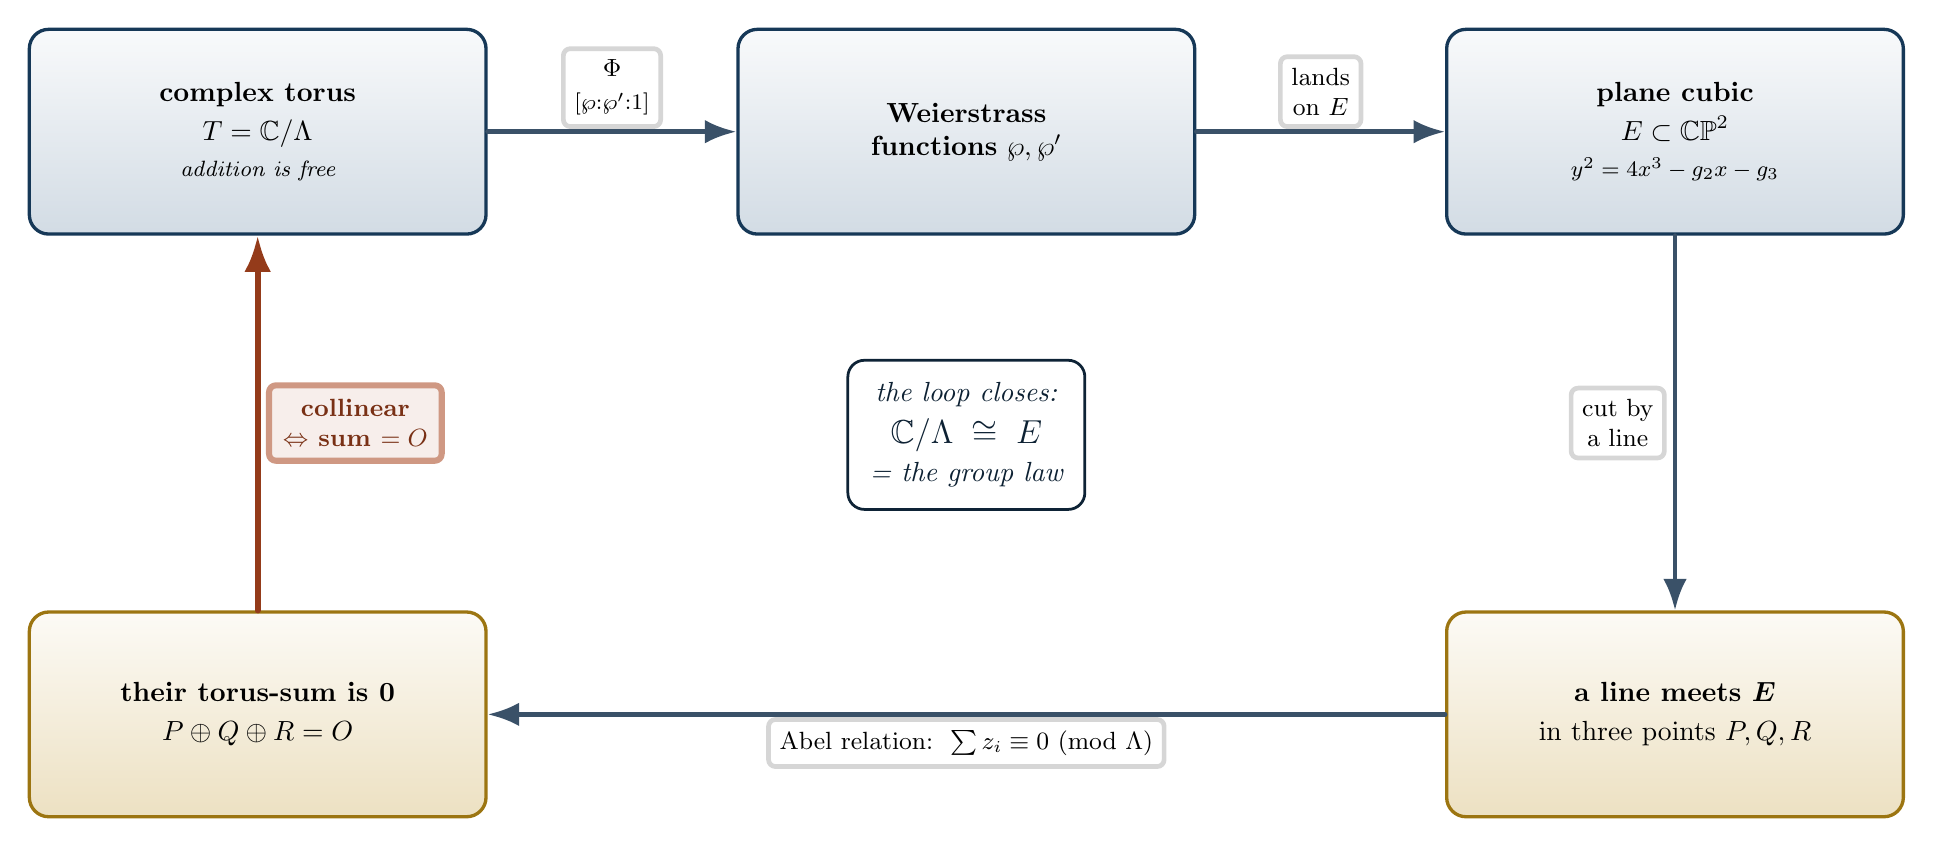
\begin{tikzpicture}[
    >=Latex, line cap=round, line join=round,
    obj/.style={rectangle, rounded corners=7pt, draw=formteal!72!black, line width=1.2pt,
      top color=formteal!3, bottom color=formteal!20, align=center,
      inner sep=9pt, minimum width=5.8cm, minimum height=2.6cm},
    fact/.style={rectangle, rounded corners=7pt, draw=formgold!85!black, line width=1.2pt,
      top color=formgold!4, bottom color=formgold!26, align=center,
      inner sep=9pt, minimum width=5.8cm, minimum height=2.6cm},
    flow/.style={-{Latex[length=4mm,width=3mm]}, line width=1.7pt, draw=formslate},
    back/.style={-{Latex[length=4.6mm,width=3.4mm]}, line width=2.2pt, draw=formrust!88!black},
    chip/.style={fill=white, draw=black!16, rounded corners=2.5pt, inner sep=4pt,
      font=\small, align=center},
    achip/.style={fill=formrust!9, draw=formrust!55, rounded corners=2.5pt, inner sep=5pt,
      font=\small\bfseries, text=formrust!72!black, align=center},
  ]
  % --- the three spaces (top row) ---
  \node[obj] (T)  at (0,0)  {\textbf{complex torus}\\[2pt]$T=\C/\Lambda$\\[1pt]{\footnotesize\itshape addition is free}};
  \node[obj] (wp) at (9,0)  {\textbf{Weierstrass}\\\textbf{functions} $\wp,\wp'$};
  \node[obj] (E)  at (18,0) {\textbf{plane cubic}\\[2pt]$E\subset\CP^2$\\[1pt]{\footnotesize$y^2=4x^3-g_2x-g_3$}};
  % --- the two mechanisms (bottom row) ---
  \node[fact] (line) at (18,-7.4) {\textbf{a line meets }$\boldsymbol{E}$\\[2pt]in three points $P,Q,R$};
  \node[fact] (div)  at (0,-7.4)  {\textbf{their torus-sum is }$\boldsymbol{0}$\\[2pt]$P\oplus Q\oplus R=O$};
  % --- central tie: a focal badge linking the two rows ---
  \node[rounded corners=6pt, draw=formteal!45!black, line width=1pt, align=center,
        fill=white, fill opacity=0.9, text opacity=1, inner sep=8pt, text=formteal!42!black]
        at (9,-3.85)
    {\itshape the loop closes:\\[3pt]{\large$\C/\Lambda\;\cong\;E$}\\[2pt]\itshape= the group law};
  % --- arrows around the loop ---
  \draw[flow] (T)  -- node[chip,above=1pt] {$\Phi$\\[1pt]{\footnotesize$[\wp{:}\wp'{:}1]$}} (wp);
  \draw[flow] (wp) -- node[chip,above=1pt] {lands\\on $E$} (E);
  \draw[flow] (E)  -- node[chip,left=3pt] {cut by\\a line} (line);
  \draw[flow] (line) -- node[chip,below=1pt] {Abel relation:\ \ $\sum z_i\equiv 0 \ (\mathrm{mod}\ \Lambda)$} (div);
  \draw[back] (div) -- node[achip,right=3pt] {collinear\\$\Leftrightarrow$ sum $=O$} (T);
\end{tikzpicture}
}\par}
\end{minipage}\hfill
\begin{minipage}[c]{0.46\linewidth}
\normalsize
The torus has an effortless addition. The bridge $\Phi$ carries it to the cubic. A
\emph{line} meets the cubic in three points whose torus-sum is $0$ --- and that single loop
\emph{is} the chord--tangent law. The three columns below walk it in order:
\par\smallskip
\textbf{(1--2)} the two characters --- torus and elliptic functions;\\
\textbf{(3--4)} the bridge --- the Weierstrass $\wp$ and the embedding;\\
\textbf{(5--6)} the payoff --- ``line, then reflect,'' and why one object wears three faces.
\end{minipage}}

\begin{columns}

%========================= COLUMN 1: the two characters =========================
\column{0.33}

\block{\large \textbf{1.} The torus $\C/\Lambda$: addition you already know}{%
\normalsize
A \emph{lattice} $\Lambda=\Z\omega_1+\Z\omega_2$ is a grid of parallelograms tiling the
plane $\C$. Glue the opposite edges of one tile and you get a \textbf{torus} (a donut
surface) $T=\C/\Lambda$: a point of $T$ is just a complex number ``read modulo the grid.''
\par\medskip
\textbf{Its addition is free.} Add the two complex numbers and wrap around:
\[ [u]\,\oplus\,[v]\;=\;[\,u+v\,]. \]
This inherits everything from $\C$: commutative and associative, identity $[0]$, inverse
$[-z]$. \emph{No geometry, no effort --- the torus is already a perfect abelian group.}
\figH{162pt}{% Addition on the torus C/Lambda: lift u and v, add as complex numbers (the dashed
% parallelogram), then wrap back into the fundamental tile by subtracting a period.
% [u]+[v] = [u+v].  Here u+v lands in the neighbouring tile and reduces by -omega_1.
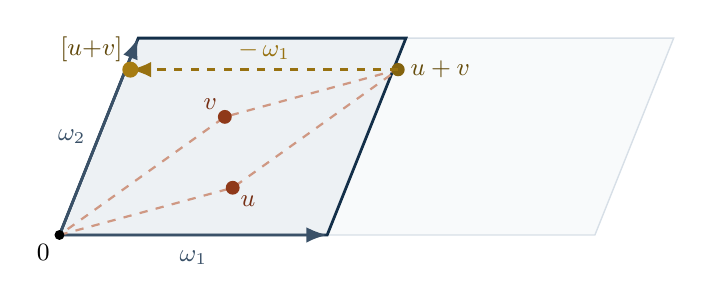
\begin{tikzpicture}[>=Latex]
  \def\ax{3.4}\def\ay{0}\def\bx{1.0}\def\by{2.5}
  % the neighbouring tile to the right (where the lifted sum lands), faint
  \draw[formteal!18, line width=0.5pt, fill=formteal!3]
    (\ax,0)--(2*\ax,0)--(2*\ax+\bx,\by)--(\ax+\bx,\by)--cycle;
  % the fundamental tile
  \draw[formteal!60!black, line width=1pt, fill=formteal!8]
    (0,0)--(\ax,\ay)--(\ax+\bx,\ay+\by)--(\bx,\by)--cycle;
  % basis vectors
  \draw[->, formslate, line width=1pt] (0,0)--(\ax,\ay) node[midway, below=2pt, font=\small] {$\omega_1$};
  \draw[->, formslate, line width=1pt] (0,0)--(\bx,\by) node[midway, left=1pt, font=\small] {$\omega_2$};
  % u, v and their lifted sum
  \coordinate (O) at (0,0);
  \coordinate (u) at (2.2,0.6);
  \coordinate (v) at (2.1,1.5);
  \coordinate (s) at (4.3,2.1);   % u+v
  \coordinate (sr) at (0.9,2.1);  % (u+v) - omega_1, reduced into the fundamental tile
  \draw[formrust!55, line width=0.8pt, dashed] (O)--(u)--(s)--(v)--cycle;
  \fill[formrust!85!black] (u) circle (2.5pt) node[below right=-1pt, font=\small, formrust!70!black] {$u$};
  \fill[formrust!85!black] (v) circle (2.5pt) node[above left=-1pt, font=\small, formrust!70!black] {$v$};
  \fill[formgold!72!black] (s) circle (2.4pt) node[right=1pt, font=\small, formgold!55!black] {$u+v$};
  % wrap back by a period
  \draw[->, formgold!82!black, line width=1pt, dashed] (s)--(sr)
    node[midway, above, font=\small] {$-\,\omega_1$};
  \fill[formgold!90!black] (sr) circle (2.9pt) node[above left=-1pt, font=\small, formgold!52!black] {$[u{+}v]$};
  \fill[black] (O) circle (1.8pt) node[below left, font=\small] {$0$};
\end{tikzpicture}
}
\figcap{To add: form $u+v$ in $\C$ (dashed), then wrap back into the tile by a period.
$[u]\oplus[v]=[u+v]$.}
\figH{185pt}{\begin{tikzpicture}\drawprecisetorus\end{tikzpicture}}
\figcap{The same tiling, glued into the torus surface --- the group we transport.}}

\block{\large \textbf{2.} Elliptic functions: rigid by Liouville}{%
\normalsize
To compare the torus with a curve we need \emph{functions on the torus} --- functions on
$\C$ that repeat on the grid, $f(z+\omega)=f(z)$. These are \textbf{elliptic functions},
and they are astonishingly rigid.
\par\smallskip
\emph{Why rigid?} A doubly periodic function with no poles is bounded, so by Liouville's
theorem it is \textbf{constant}. Hence any non-constant one \emph{must} have poles --- and
integrating around one tile (opposite sides cancel) shows it has as many poles as zeros.
The very simplest possible has a single double pole.
\callout{formgold}{The seed.}{Even the \emph{positions} are pinned down: integrating
$z\,f'(z)/f(z)$ around a tile gives the \textbf{Abel relation}
\[ \sum(\text{zeros})-\sum(\text{poles})\in\Lambda . \]
This one fact is what forces the reflection step at the very end.}
The function realising the simplest case --- one double pole, nothing else --- is the
\emph{Weierstrass} $\wp$, built next.
\figH{202pt}{% One tile of the lattice with the boundary traversed counterclockwise.
% Integrating f, f'/f, z f'/f around it: opposite sides carry equal values (f is doubly
% periodic) and cancel -- this is Liouville's count (#zeros = #poles) and the Abel relation.
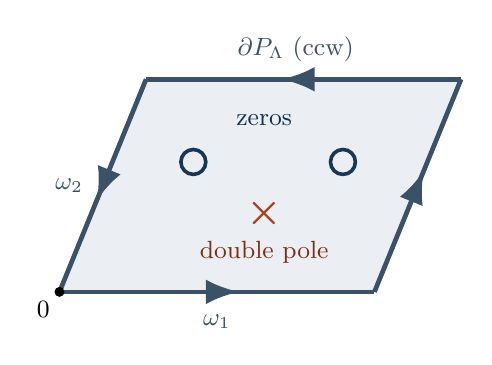
\begin{tikzpicture}[>=Latex,
    edge/.style={formslate, line width=1.7pt, postaction={decorate},
      decoration={markings, mark=at position 0.57 with {\arrow{Latex[length=4.2mm]}}}}]
  \def\ax{4.0}\def\bx{1.1}\def\by{2.7}
  \fill[formteal!9] (0,0)--(\ax,0)--(\ax+\bx,\by)--(\bx,\by)--cycle;
  % directed boundary contour, ccw
  \draw[edge] (0,0)--(\ax,0) node[midway, below=4pt, formslate, font=\small] {$\omega_1$};
  \draw[edge] (\ax,0)--(\ax+\bx,\by);
  \draw[edge] (\ax+\bx,\by)--(\bx,\by);
  \draw[edge] (\bx,\by)--(0,0) node[midway, left=3pt, formslate, font=\small] {$\omega_2$};
  \fill[black] (0,0) circle (1.8pt) node[below left, font=\small] {$0$};
  % label the oriented boundary, placed outside above the top edge
  \node[formslate, font=\small] at (3.0,3.08) {$\partial P_\Lambda$ (ccw)};
  % two zeros and a double pole, stacked with clear vertical separation
  \node[formteal!60!black, font=\small] at (2.6,2.18) {zeros};
  \draw[formteal!70!black, line width=1.3pt] (1.7,1.65) circle (4.5pt);
  \draw[formteal!70!black, line width=1.3pt] (3.6,1.65) circle (4.5pt);
  \node[formrust, font=\Large] at (2.6,1.0) {$\boldsymbol\times$};
  \node[formrust!72!black, font=\small] at (2.6,0.5) {double pole};
\end{tikzpicture}
}
\figcap{Integrate $f,\ f'/f,\ z\,f'/f$ counterclockwise around one tile $\partial P_\Lambda$.
Opposite sides carry equal values ($f$ repeats), so they cancel --- forcing
$\#$zeros $=\#$poles and the Abel relation
$\sum(\text{zeros})-\sum(\text{poles})\in\Lambda$.}}

%========================= COLUMN 2: the bridge =========================
\column{0.33}

\block{\large \textbf{3.} The Weierstrass function $\wp$: the simplest one}{%
\normalsize
To \emph{build} an elliptic function with a single double pole, sum $1/z^2$ over the whole
lattice (with constants for convergence):
\[ \wp(z)=\frac{1}{z^2}+\!\!\sum_{\lambda\in\Lambda\setminus 0}\!\!
   \Big(\frac{1}{(z-\lambda)^2}-\frac{1}{\lambda^2}\Big). \]
It is even, one double pole per tile; its derivative $\wp'$ is odd, with a triple pole.
\figH{160pt}{% Why wp has a double pole at every lattice point: it is the sum  sum_lambda (z-lambda)^-2
% over the whole lattice.  A grid of double-pole markers, with a sample point z receiving
% its dominant contributions from the four nearest lattice points.
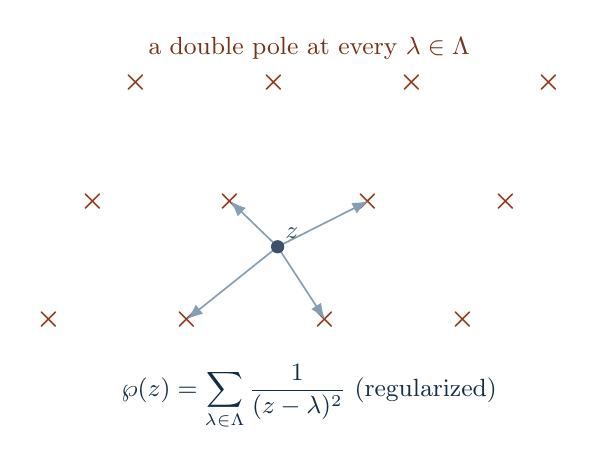
\begin{tikzpicture}[>=Latex]
  \def\ax{1.75}\def\bx{0.55}\def\by{1.5}
  \foreach \i in {-1,0,1,2}{\foreach \j in {0,1,2}{
    \node[formrust!85!black] at (\i*\ax+\j*\bx,\j*\by) {$\boldsymbol\times$};}}
  \coordinate (z) at (1.15,0.92);
  \foreach \px/\py in {0/0, 1.75/0, 0.55/1.5, 2.30/1.5}{
    \draw[formteal!55, line width=0.6pt, ->] (z)--(\px,\py);}
  \fill[formslate] (z) circle (2.4pt);
  \node[formslate, font=\small, above right=-1pt] at (z) {$z$};
  \node[formrust!72!black, font=\small, anchor=south] at (1.55,3.18)
    {a double pole at every $\lambda\in\Lambda$};
  \node[formteal!58!black, font=\small, anchor=north] at (1.55,-0.45)
    {$\displaystyle \wp(z)=\sum_{\lambda\in\Lambda}\frac{1}{(z-\lambda)^2}$ (regularized)};
\end{tikzpicture}
}
\figcap{The sum runs over the whole lattice, planting a double pole at every $\lambda$; near
$z$ the four closest terms dominate.}
\par\medskip
\textbf{One magic identity.} Near $0$, $\wp=z^{-2}+3G_4z^2+\cdots$, so $\wp'^2$ and
$4\wp^3$ \emph{both} begin with $4z^{-6}$. Subtract them and the right multiples of $\wp$
and $1$: every pole cancels, leaving a bounded --- hence constant --- function. So $\wp$
and $\wp'$ satisfy one cubic relation:
\[ \boxed{\;\wp'^2 = 4\wp^3 - g_2\,\wp - g_3\;}\qquad g_2=60G_4,\ \ g_3=140G_6. \]
\figH{188pt}{% The Weierstrass function on the real axis: a double pole at every lattice point, even,
% with one valley per period bottoming out at a real root e_1.  (Drawn from a truncated
% lattice sum, plotted on pole-avoiding sub-intervals so values stay on-scale.)
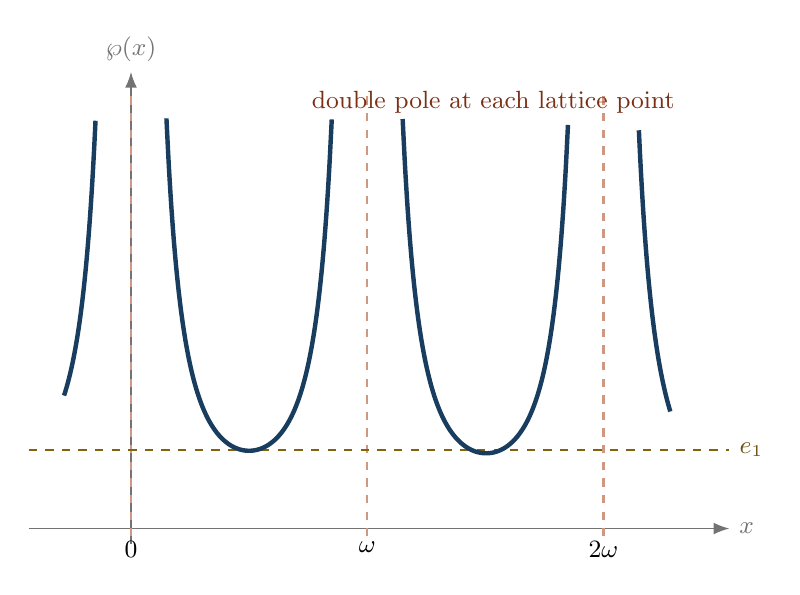
\begin{tikzpicture}[>=Latex]
  \draw[->, black!55, line width=0.6pt] (-1.3,0)--(7.6,0) node[right, font=\small] {$x$};
  \draw[->, black!55, line width=0.6pt] (0,-0.2)--(0,5.8) node[above, font=\small] {$\wp(x)$};
  % vertical asymptotes at the lattice points
  \foreach \p in {0,3,6}{\draw[formrust!55, dashed, line width=0.8pt] (\p,-0.1)--(\p,5.55);}
  % the level of the real root reached at the half-period
  \draw[formgold!72!black, dashed, line width=0.7pt]
    (-1.3,1)--(7.6,1) node[right, font=\small, formgold!58!black] {$e_1$};
  % the graph, drawn on intervals that keep a safe margin from each pole
  \foreach \lo/\hi in {-0.85/-0.45, 0.45/2.55, 3.45/5.55, 6.45/6.85}{
    \draw[formteal!78!black, line width=1.6pt, smooth, samples=70, domain=\lo:\hi]
      plot (\x, {1/((\x)^2) + 1/((\x-3)^2) + 1/((\x+3)^2) + 1/((\x-6)^2)});}
  \node[below, font=\small] at (0,-0.04) {$0$};
  \node[below, font=\small] at (3,-0.04) {$\omega$};
  \node[below, font=\small] at (6,-0.04) {$2\omega$};
  \node[formrust!72!black, font=\small, anchor=south] at (4.6,5.15) {double pole at each lattice point};
\end{tikzpicture}
}
\figcap{On the real axis $\wp$ has a double pole at every lattice point and one valley per
period, bottoming at a real root $e_1=\wp(\omega/2)$ --- the picture behind ``a single
double pole.''}}

\block{\large \textbf{4.} The bridge $\Phi$: drawing the torus as a cubic}{%
\normalsize
Now send each torus point to the projective point
\[ \Phi(z)=[\wp(z):\wp'(z):1],\qquad \Phi(0)=O=[0{:}1{:}0]. \]
The boxed identity puts the image on the cubic $E:\,y^2=4x^3-g_2x-g_3$, and in fact $\Phi$
is a biholomorphism $\C/\Lambda\xrightarrow{\,\sim\,}E$. \emph{Why a bijection?} $\wp$ is
$2$-to-$1$ (it is even), and $\wp'$ tells the two preimages apart by its sign --- the
branched cover below.
\figH{216pt}{\begin{tikzpicture}[scale=1.0, every node/.style={font=\small}]
  % Top: precise torus with the four 2-torsion (half-lattice) points marked.
  \begin{scope}[yshift=2.0cm, scale=0.85]
    \drawprecisetorus
    \fill[formrust!85!black] (\torusMarkhalfsumx,\torusMarkhalfsumy) circle (3pt);
    \node[formrust!60!black, above, font=\scriptsize]
      at (\torusMarkhalfsumx,\torusMarkhalfsumy) {$[\tfrac{\omega_1+\omega_2}{2}]$};
    \fill[formrust!85!black] (\torusMarkzerox,\torusMarkzeroy) circle (3pt);
    \node[formrust!60!black, below right, font=\scriptsize]
      at (\torusMarkzerox,\torusMarkzeroy) {$[\tfrac{\omega_1}{2}]$};
    \fill[formrust!85!black] (\torusMarkhalftwox,\torusMarkhalftwoy) circle (3pt);
    \node[formrust!60!black, below left, font=\scriptsize]
      at (\torusMarkhalftwox,\torusMarkhalftwoy) {$[\tfrac{\omega_2}{2}]$};
    \fill[formrust!85!black] (\torusMarkhalfonex,\torusMarkhalfoney) circle (3pt);
    \node[formrust!60!black, right, font=\scriptsize]
      at (\torusMarkhalfonex,\torusMarkhalfoney) {$[0]$};
    \node[formteal!55!black] at (-3.0,1.0) {$T$};
  \end{scope}
  \draw[-{Latex[length=3mm]}, formplum, line width=1.1pt] (0,0.7) -- (0,-0.1);
  \node[formplum] at (0.35,0.3) {$\wp$, deg 2};
  \begin{scope}[yshift=-1.5cm, scale=1.1]
    \drawprecisesphere
    \fill[formrust!85!black] (\sphereNorthx,\sphereNorthy) circle (2.4pt);
    \node[formrust!60!black, above, font=\scriptsize]
      at (\sphereNorthx,\sphereNorthy) {$\infty$};
    \fill[formrust!85!black] (-0.707,-0.354) circle (2.4pt);
    \node[formrust!60!black, left, font=\scriptsize] at (-0.78,-0.354) {$e_1$};
    \fill[formrust!85!black] (0,-0.500) circle (2.4pt);
    \node[formrust!60!black, below, font=\scriptsize] at (0,-0.56) {$e_2$};
    \fill[formrust!85!black] (0.707,-0.354) circle (2.4pt);
    \node[formrust!60!black, right, font=\scriptsize] at (0.78,-0.354) {$e_3$};
    \node[formteal!55!black] at (-1.65,0.6) {$\CP^1$};
  \end{scope}
  \node[draw=black!40, rounded corners=2pt, fill=formivory, align=left, anchor=west,
        inner sep=4pt] at (3.4,0.4)
    {The map $\wp:T\to\CP^1$ is a\\$2:1$ branched cover\\
     with $4$ branch values:\\
     three roots $e_1,e_2,e_3$ and $\infty$.\\
     Riemann--Hurwitz:\\
     $0=2{\cdot}2-4{\cdot}(2-1)$.};
\end{tikzpicture}
}
\figcap{$\wp:T\to\CP^1$ folds the torus $2$-to-$1$ onto the sphere, branching only over the
three roots $e_1,e_2,e_3$ and $\infty$. Recording $\wp'$ as well unfolds it into the cubic
$E$ --- a flawless dictionary $T\cong E$.}
\callout{formteal}{Now the payoff.}{We have a perfect dictionary $T\cong E$. \emph{Transport
the torus's effortless addition through $\Phi$} --- what does it become on the curve?}}

%========================= COLUMN 3: payoff, example, outlook =========================
\column{0.34}

\block{\large \textbf{5.} The payoff: addition becomes ``line, then reflect''}{%
\normalsize
Here is the one fact behind it all. A line $ax+by+c=0$ pulls back to $a\wp+b\wp'+c$, an
elliptic function with a \emph{single triple pole} at $O$ --- so exactly three zeros, which
(by Abel) sum to $0$ on the torus:
\[ P,Q,R\ \text{collinear on }E\ \Longleftrightarrow\ P\oplus Q\oplus R=O. \]
Thus $P\oplus Q=\ominus R$. And $\ominus$ on the torus is $z\mapsto-z$, i.e.\
$(x,y)\mapsto(x,-y)$ ($\wp$ even, $\wp'$ odd) --- \textbf{reflection across the $x$-axis}.
Mystery solved.
\figH{200pt}{% Chord law on E: y^2 = 4x^3 - 4x, using Sage-computed chord coordinates.
\begin{tikzpicture}[scale=1.0, every node/.style={font=\small}]
  \draw[->, black!45, line width=0.5pt] (-1.7,0) -- (2.7,0) node[right, black!55] {$x$};
  \draw[->, black!45, line width=0.5pt] (0,-3.3) -- (0,3.5) node[above, black!55] {$y$};
  \drawprecisecurve
  \foreach \rt in {\rooteone,\rootetwo,\rootethree}
    \fill[formteal!60!black] (\rt,0) circle (1.4pt);
  \draw[draw=formplum, line width=0.9pt] (\chordlefta,\chordleftb) -- (\chordrighta,\chordrightb);
  \draw[dashed, line width=0.5pt, formgold!75!black] (\chordRx,\chordRy) -- (\chordSx,\chordSy);
  \fill[formrust!85!black] (\chordPx,\chordPy) circle (2.4pt);
  \node[formrust!60!black, above left]  at (\chordPx,\chordPy) {$P$};
  \fill[formrust!85!black] (\chordQx,\chordQy) circle (2.4pt);
  \node[formrust!60!black, above right] at (\chordQx,\chordQy) {$Q$};
  \fill[formteal!85!black] (\chordRx,\chordRy) circle (2.4pt);
  \node[formteal!60!black, above left]  at (\chordRx,\chordRy) {$R$};
  \fill[formgold!85!black] (\chordSx,\chordSy) circle (2.8pt);
  \node[formgold!50!black, below left]  at (\chordSx,\chordSy) {$P\oplus Q=-R$};
\end{tikzpicture}
}
\figcap{The line through $P$ and $Q$ meets $E$ at a third point $R$; reflecting $R$ across
the $x$-axis gives $P\oplus Q$. Collinear means torus-sum $0$; reflection is $z\mapsto-z$.}}

\block{\large \textbf{6.} Why it matters: one object, three faces}{%
\normalsize
What we built is a single abelian group seen three ways --- and the isomorphisms between
those views \emph{are} the subject:
\[ \underbrace{\C/\Lambda}_{\text{analysis}}\ \cong\
   \underbrace{\Pic^0(E)}_{\text{geometry}}\ \cong\
   \underbrace{E(k)}_{\text{arithmetic}}. \]
\callout{formgold}{Three faces.}{\textbf{Analytic} --- $\C/\Lambda$: complex numbers added
modulo a lattice.\\ \textbf{Geometric} --- $\Pic^0(E)$: degree-$0$ divisor classes (line
bundles); Abel--Jacobi makes $E$ its own Jacobian.\\ \textbf{Arithmetic} --- $E(k)$: the
points themselves, under chord--tangent, over \emph{any} field $k$.}
That last face is the doorway to modern number theory: because the law is \emph{rational},
it travels to every field at once.
\par\smallskip
\textbf{Over $\Q$.}\ \ Mordell--Weil: $E(\Q)\cong\Z^{r}\oplus E(\Q)_{\mathrm{tors}}$ is
finitely generated. The \emph{rank} $r$ is deep --- Birch--Swinnerton-Dyer (a Clay
Millennium Prize problem) predicts it from the order of vanishing of the $L$-function
$L(E,s)$ at $s=1$.
\par\smallskip
\textbf{Over $\F_p$.}\ \ Hasse's bound $\bigl|\#E(\F_p)-(p+1)\bigr|\le 2\sqrt p$ pins the
point count, and the hardness of \emph{reversing} the group law underwrites
elliptic-curve cryptography.
\par\smallskip
\textbf{Galois \& modularity.}\ \ The torsion assembles into a representation
$\rho:\operatorname{Gal}(\overline\Q/\Q)\to\mathrm{GL}_2(\Z_\ell)$; every $E/\Q$ is
\emph{modular} --- the theorem behind Wiles's proof of Fermat's Last Theorem.
\par\smallskip
And $j=1728\,g_2^3/\Delta$ names the curve inside the moduli space of \emph{all} elliptic
curves --- the next picture:
\figH{172pt}{% The moduli space of complex tori: a torus C/Lambda depends only on its shape
% tau in H, modulo SL_2(Z).  The shaded region F (|Re tau|<=1/2, |tau|>=1) is one
% representative per torus; H/SL_2(Z) is coordinatized by the j-invariant.  The faint
% geodesics and walls suggest the SL_2(Z) tessellation.
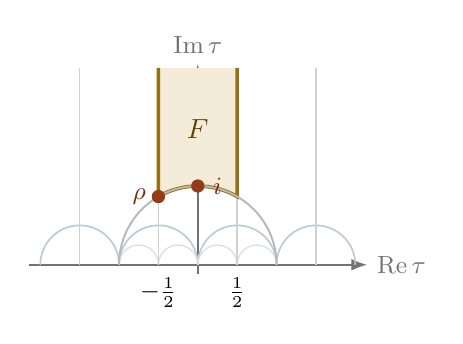
\begin{tikzpicture}[>=Latex]
  \def\rt{0.86603}
  \draw[->, black!55, line width=0.6pt] (-2.15,0)--(2.15,0) node[right, font=\small] {$\operatorname{Re}\tau$};
  \draw[->, black!55, line width=0.6pt] (0,-0.12)--(0,2.55) node[above, font=\small] {$\operatorname{Im}\tau$};
  % tessellation: integer-to-integer geodesics, then half-integer ones, fainter
  \foreach \a/\b in {-2/-1,-1/0,0/1,1/2}{
    \pgfmathsetmacro\c{(\a+\b)/2}\pgfmathsetmacro\rr{(\b-\a)/2}
    \draw[formteal!30, line width=0.6pt] (\c+\rr,0) arc[start angle=0, end angle=180, radius=\rr];}
  \foreach \a/\b in {-1/-0.5,-0.5/0,0/0.5,0.5/1}{
    \pgfmathsetmacro\c{(\a+\b)/2}\pgfmathsetmacro\rr{(\b-\a)/2}
    \draw[formteal!17, line width=0.5pt] (\c+\rr,0) arc[start angle=0, end angle=180, radius=\rr];}
  % neighbour walls (faint)
  \foreach \x in {-1.5,-0.5,0.5,1.5}{\draw[black!18, line width=0.5pt] (\x,0)--(\x,2.5);}
  % fundamental domain F
  \fill[formgold!16] (-0.5,2.5)--(-0.5,\rt) arc[start angle=120, end angle=60, radius=1]--(0.5,2.5)--cycle;
  \draw[formgold!82!black, line width=1.3pt]
    (-0.5,2.5)--(-0.5,\rt) arc[start angle=120, end angle=60, radius=1]--(0.5,2.5);
  % unit circle, faint
  \draw[black!28, line width=0.7pt] (1,0) arc[start angle=0, end angle=180, radius=1];
  % distinguished points and labels
  \fill[formrust!88!black] (0,1) circle (2.4pt);
  \node[right=2pt, font=\small, formrust!70!black] at (0,1) {$i$};
  \fill[formrust!88!black] (-0.5,\rt) circle (2.4pt);
  \node[left=1pt, font=\small, formrust!70!black] at (-0.5,\rt) {$\rho$};
  \node[formgold!50!black] at (0,1.72) {$F$};
  \node[below, font=\small] at (-0.5,-0.04) {$-\tfrac12$};
  \node[below, font=\small] at (0.5,-0.04) {$\tfrac12$};
\end{tikzpicture}
}
\figcap{$F$ is one representative per torus, so $\HH/\mathrm{SL}_2(\Z)$ is the moduli space
of complex tori --- coordinate the $j$-invariant; $i,\rho$ are the extra-symmetric tori.}
\par\smallskip
{\footnotesize\textbf{Author:} \(\langle\)Your Name\(\rangle\) \,\textbullet\,
\(\langle\)email\(\rangle\) \,\textbullet\, seeking PhD positions in arithmetic \& algebraic
geometry. \;From the textbook \emph{Complex Tori and Elliptic Curves} (self-contained;
${\sim}80$ solved exercises).}}

\end{columns}
\end{document}
